
\chapter{Vue d'ensemble du système}\label{ch:systeme}

Le système est composé de plusieurs acteurs différents qui ont chacun une tâche bien précise, ce chapitre propose une vue d'ensemble de ses éléments et explique également les interactions qu'ils existent entre eux.

L'objectif du système est de permettre la récupération de toutes les données récoltées par le ou les capteurs et de centraliser ces informations afin que l'application mobile puisse les exploiter et les afficher aux utilisateurs au travers de son interface graphique.

Afin de pouvoir réaliser cet objectif, les éléments suivants sont développés.

\begin{itemize}
\item Un capteur
\item Une passerelle
\item Une base de données
\item Une application mobile
\end{itemize}

Le capteur est porté par un sportif, il est en charge de l'acquisition des données et de leur transmissions à une passerelle en utilisant la couche radio LoRa. Il est définit en détails dans le chapitre~\ref{ch:capteur}.

La passerelle se charge de récupérer les données transmises par le ou les capteurs, les traites et puis les centralises dans une base de données. Elle est décrite dans le chapitre~\ref{ch:passerelle}.

La base de données permet le stockage de toutes les informations collectées durant la course mais également d'autres informations qui sont saisies avant, comme le nom et prénom, le numéro de dossard ou le pays d'origine des athlètes. Chaque compétition ainsi que leurs informations associées sont également enregistrées dedans. Le chapitre~\ref{ch:bd} explique son fonctionnement.

L'application mobile est la fenêtre sur le système, elle permet aux utilisateurs de visualiser en temps réel l'évolution de la course. Sa description se trouve dans le chapitre~\ref{ch:app_mobile}.

Afin de pouvoir être utilisable pendant des compétitions sportives, le système doit être capable de gérer plusieurs capteurs en parallèle, il est donc développé dans cette optique. Cependant dans la mesure ou dans le cadre du travail de Bachelor le projet est une preuve de concept, un seul capteur sera assemblé et testé. 

En ce qui concerne les passerelles, idéalement plusieurs d'entre elles doivent pouvoir être utilisées durant une course, cela permet de diminuer les zones d'ombres le long du parcours et également de minimiser le nombre de paquets perdus. Cependant cela complique passablement le système, car cela implique que la base de données doit être hébergée sur un serveur connecté à internet et donc que la passerelle doit également pouvoir s'y connecter. Afin de simplifier le développement du projet, il est décidé de ne développé qu'une seule passerelle et d'y héberger localement la base de données.

Enfin le chapitre~\ref{ch:produit} rassemble les éléments qu'il faudrait retravailler afin de faire de la preuve de concept un produit à part entière.

\section{Les interactions}

Le système exploite deux types de communication différentes afin de stocker et d'extraire des données de la base. D'une part la couche radio LoRa est utilisée pour la communication entre les capteurs et les passerelles, et d'autre part le WiFi pour les requêtes entre la base de données et l'application mobile. 

Dans le cadre de la preuve de concept et pour des raisons de simplifications, la couche MAC LoRaWAN n'est pas employée, elle prendrait cependant tout son sens dans une optique de développement d'un produit.

La figure~\ref{fig:system_schema} montre les interactions existantes entre les acteurs du système.

\begin{figure}[htb]
\centering 
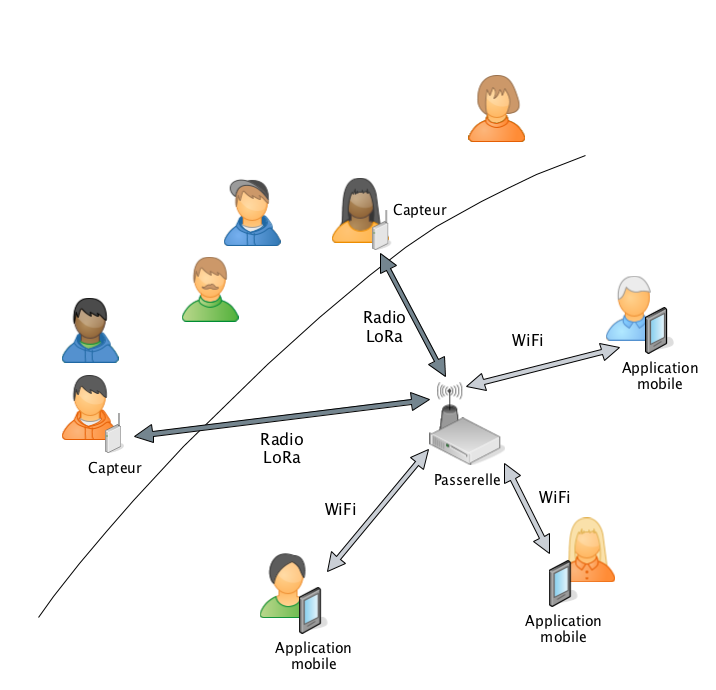
\includegraphics[width=0.9\columnwidth]{system_schema.png} 
\caption{Interactions des acteurs du système}
\label{fig:system_schema}
\end{figure}

\section{La couche radio LoRa}

\todo{}



